%CHAPTER 1: Introduction
\chapter{Introduction}

Transformers are the backbone of all the Large-Language Models (LLMs) that are present today. The concept of transformers was introduced in a ground-breaking paper titled \textbf{\href{https://proceedings.neurips.cc/paper_files/paper/2017/file/3f5ee243547dee91fbd053c1c4a845aa-Paper.pdf}{Attention is All You Need}} in 2017 by a group of researchers at \textbf{Google}. That paper brought a revolution in the field of Deep Learning. Even the researchers who published the paper had not expected that it would bring such a change in this field. \\

\begin{figure}[h]
    \centering
    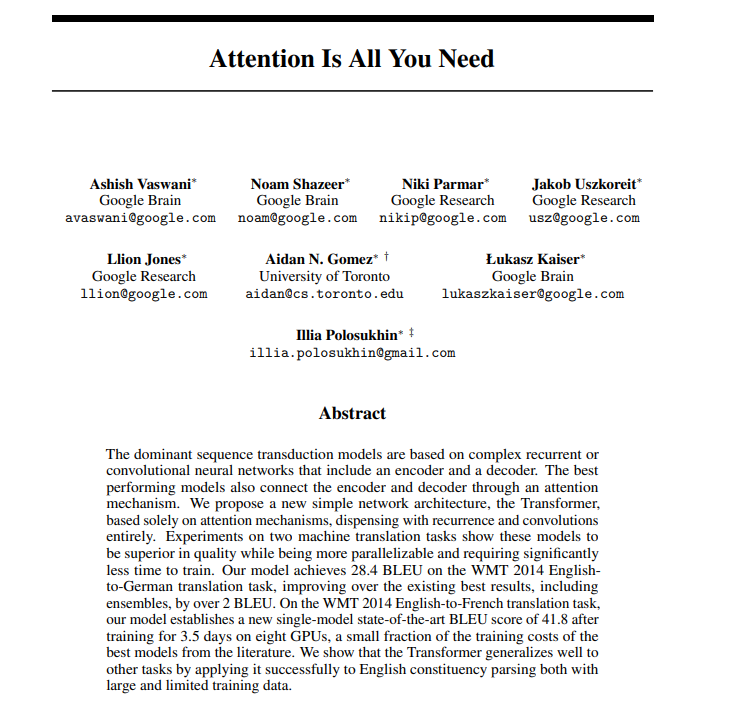
\includegraphics[width=0.5\linewidth]{Introduction/transformer-paper.png}
    \caption{The original paper on Transformers}
\end{figure}

Before moving on to a technical discussion on transformers, it will be good if we discuss a little bit about what they are and their impact on society. Going forward, this will enable us to have a better understanding of the topic. \\

%SECTION 1: What are transformers?
\section{What are transformers?}

Transformers are a neural network architecture that was created specifically for \textit{sequence-to-sequence} tasks, where both the input and the output of the task is sequential data (sentences and paragraphs). A well-known example of such tasks is \textit{machine translation}, where sentences in one language are converted into another language. That is why they are called transformers - because they transform one sequence to the other. \\

Unlike previous sequential models like \textbf{RNNs} and \textbf{LSTMs} which process inputs one-by-one (one token after another), transformers have the ability to process all tokens at once simultaneously. This makes the training process much faster and improves accuracy. The model can learn relationships between words regardless of their distance in the sentence.\\

As an example, consider the sentence \textit{"The scientist who won the award thanked her colleagues because she appreciated their support"}. The word "she" refers to "scientist," even though several words separate them. Traditional models may struggle to preserve such long-range information, whereas a Transformer can establish this connection.

% SECTION 2: Impact
\section{Impact in the field of AI and ML}

The impact of transformers in the field of AI and ML has been tremendous. Although created for sequence-sequence tasks, they have multimodal capabilities, which means that they can be used with different data types like audio, images, etc. Some of their impacts are listed:

\begin{enumerate}
    \item \textbf{Natural Language Processing:} Transformers have transformed the NLP landscape by improving performance of tasks like machine translation, text summarisation, question answering, etc.
    \item \textbf{Computer Vision:} Transformers are used with CNNs (Convolutional neural networks) to achieve state-of-the-art results in tasks like image classification, object detection, etc.
    \item \textbf{Generative AI:} Transformers are the foundation of generative AI models. They can generate human-like text, computer text, images, audio, etc. Examples include ChatGPT, Gemini, Deepseek, etc.
    \item \textbf{Multimodal AI:} Multimodal learning is where a single model can process multiple types of data. Transformers can combine text, images, audio, etc to perform tasks like generating images from text description, answering questions from images, etc.
\end{enumerate}

% SECTION 3: Objectives and scope
\section{Objectives and scope of the report}

This report will provide a deep dive into the internal architecture of a Transformer and how it works. We will first cover the components used in the architecture like self-attention, positional encoding and cross-attention before understanding how all of them are used together. So fasten your seat-belts and get ready for an exciting journey into the world of transformers!